%!TEX root = ../../main.tex
\section{Administration Tools}\label{sec:impAdminTools}
% This section describes the administrative functionality. 
% It covers route history, GPS history, bicycle usage history, and an add/remove page.
% It also contains a bicycle GPS tracking, but this has been mentioned in \secref{sec:googlemapsapi}.
In \secref{sec:designAdminTools} some questions were asked. 
In this section we answer these questions.
To answer the question about which routes are used we implemented a feature to show route history, which can be seen in \secref{sec:routeHistory}.
Hotspot detection was not implemented, but GPS history was implemented in \secref{sec:gpsHistory}.
The traffic og bicycles during some period and the current amount of bicycles at a given station can be seen using the implemented graph in \secref{sec:bicycleUsageHistory}.
How the amount of bicycles at a station change over time can be seen in the same graph.

\subsection{Route History}\label{sec:routeHistory}
This part of the administration site handles showing a map of the historical locations of a bicycle.
The admin provides one or more bicycles, a start, and end date.
Then if there are historical GPS coordinates for the bicycle(s), they will be shown on the map. 

The purpose of the route history page is to give the admins an idea of which roads the bicycles are traveling a lot on. 
This can then be used as a decision-making tool to decide where to put new stations, in that if the admin can see that a lot of bicycles are traveling to a specific point it might be a good idea to put a station there.
It could also be used to see if a specific bicycle is being 'misused' in the sense that it would be visible if the bicycle is only being used to travel to one spot and nowhere else.

See \figref{fig:routehistory} for a figure of what the page looks like.

\begin{figure}[H]
	\centering
	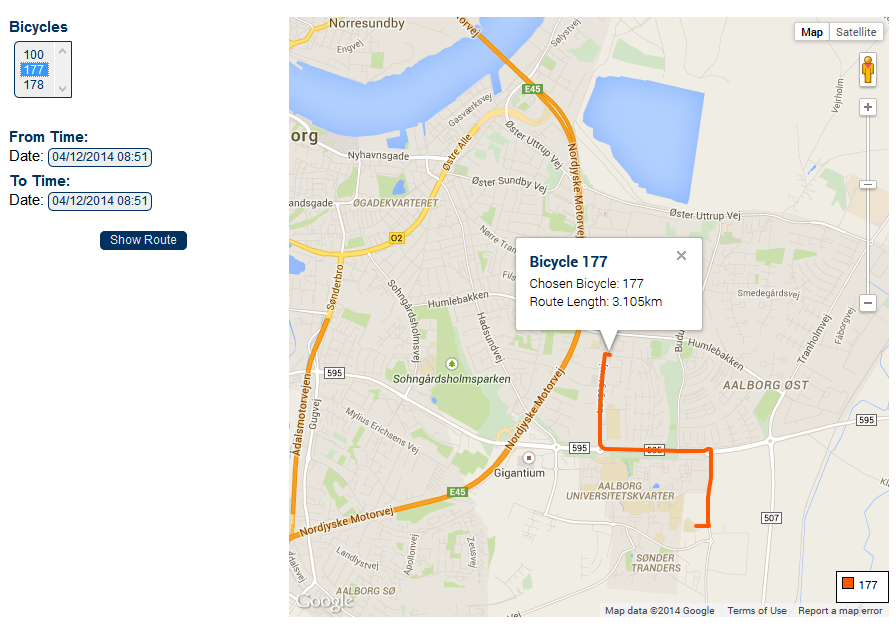
\includegraphics[scale=0.75]{RouteHistory.png}
	\caption{Picture of Route History}
	\label{fig:routehistory}
\end{figure}

From the figure, the presentation of routes are shown for the bicycles with id 36 and 95.
The reason multiple bicycles can be selected is to enable the admin to compare routes on the same map, this includes the route polyline, chosen bicycle and length,

It is implemented by finding all the bicycles that have associated historical GPS data.
 The administrator then chooses which bicycles to map, and these bicycles then have their routes loaded which are then given to Google Maps API to display.


\subsection{GPS History}\label{sec:gpsHistory}
The system saves the location of bicycles registered in the system, which could be helpful for determining where bicycles currently are. 
This would allow the 'county' to determine where 'lost' bicycles are, which in turn would allow for easier recovery of bicycles.
Having the GPS tracking already implemented, it makes sense to store the GPS coordinates in a separate table for historical and business intelligence purposes.
This kind of historical data could be interesting for intelligence purposes because it would allow knowledge about the following:

\begin{description}[style=nextline]
\item[Which routes are used?] If routes could be determined, patterns could possibly be seen, e.g. if there is a particular route that is very popular.
\item[Are there hotspots for bicycles?] If positions of bicycles could be determined, it would mean that hotspots(places where there is a lot of bicycle activity) could be found. 
This could provide valuable knowledge about for example where to add new stations.
\end{description}

A table to store this is created, containing the following information:

\begin{itemize}
\item The ID of the Bicycle
\item A timestamp of when the coordinates was recorded.
\item The latitude and the longitude.
\end{itemize}

At the same time when location is recorded from a service, it needs to also record it permanently in the global database.

\subsection{Bicycle Usage History}\label{sec:bicycleUsageHistory}
% Disposition:
% What does it track?
% Which questions can be answered?
% How is it implemented?

Besides recording the exact location of each bicycle with GPS coordinates, the system also records the stations a given bicycle visits. 
This can be used to give an overview of the bicycle traffic between stations.
Furthermore, the amount of docked bicycles is tracked for each station, giving an overview of which stations that have high and low activity.

\begin{description}[style=nextline]
\item[Where is the most traffic of bicycles during some period?] An admin user would be able to see how many bicycles leaves and arrives at each station and thereby get an overview of where the traffic is high and low, providing an indication of where to put focus for relocation of bicycles and expansion of stations.
\item[What is the current amount of bicycles at a given station?] A graph is shown providing the amount of bicycles on the y-axis and the provided timespan on the x-axis. This gives the admin user an idea when bicycles leave each station.
\item[How does the amount of bicycles at a given station change over time?] Taking the same graph as above, the admin user can also choose a long period of time for example a week, month or a year, providing a more general overview of when the activity at each station is high or low.
\end{description}

These features are implemented through two additional tables added to the database, where the first table keeps information about the amount of bicycles at a station along with a timestamp. 
The other table keeps information about the time and station a bicycle left from and arrived to, along with the specific bicycle id and a possible booking id associated with the bicycle trip.

As this information needs to be captured and updated when an event occurs, either being a bicycle that is taken from a station dock or a bicycle return to a station dock, these operations are performed in the interface between the stations and the global database, see \figref{fig:overallarch}. 
The stations will communicate with this interface when either of these events occur. 
The timestamp is generated just before query execution, which means that some delay can occur from the actual event firing time to the insertion time, resulting in an imprecise trip duration. 
This is, however, considered a minor deviation in most cases, because the communication delay is short (seconds maybe even less).
In case of a bad connection, the generated timestamp will cause useless data in the light of statistical usage, if time is an important aspect of the analysis.
For showing the traffic between stations the timestamp is used for filtering on a specified time interval and thereby allowing up to an hour of imprecision.
This time interval is an assumed granularity and would have to be specified by the admin.
The graph showing the amount of bicycles docked at a station shows the timestamp on the x-axis, however, in this case it is considered acceptable with some imprecision since this data will not be used for statistics but for a visual overview.